% (Zhou Junyuan) The following content is not highly relevant to the main text, so it will not be included in the body.

% In this section, we will introduce the basic data types supported by \MindQuantum. When we run quantum evolution in \MindQuantum, different data types require different sizes of computer memory and lead to different simulation accuracy.
% Before we discuss the supported data types in \MindQuantum, we first briefly review the definition of the floating-point number in modern computers which helps us understand the difference among these data types.
% The first unified technical standard of floating-point arithmetic (IEEE 754) \cite{8766229} was established in 1985 and is widely supported by various hardware today by the Institute of Electrical and Electronics Engineers (IEEE).

% In IEEE 754, a floating-point format is specified by three parts, sign, exponent, and fraction, all of which consist of a ${0,1}$ bit string as shown in Fig.~\ref{fig:ieee}.

% \begin{figure}[h]
%     \centering
%     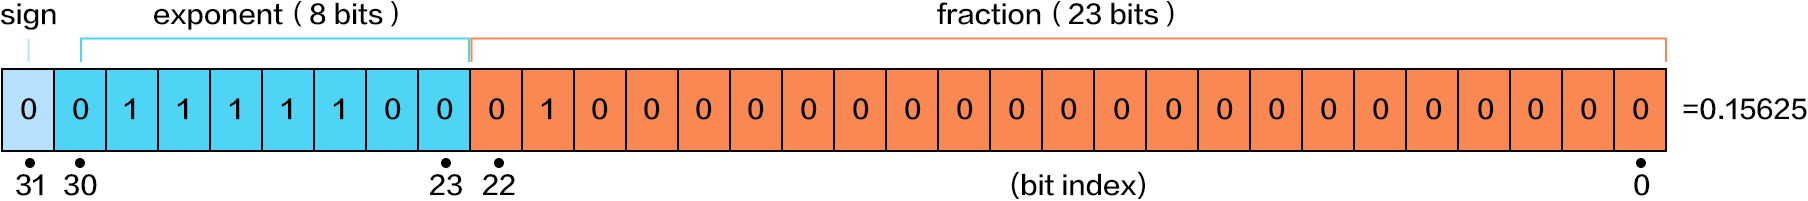
\includegraphics[width=\linewidth]{2.1_figures/Float_example.png}
%     \caption{Floating-point format}
%     \label{fig:ieee}
% \end{figure}

% The sign bit $s$ determines the sign of the number, $s=0$ is positive and $s=1$ is negative.
% The exponent part $e$ is an m-bit unsigned integer, which determines the Maximum and minimum values, and the fraction part $\vec{b}$ with $n$ bits is the true significance that appears in the memory format which determines the precision of the number.

% The real value assumed by a given sign $s$, biased exponent $e$ and fraction $\vec{b}$ as
% \begin{equation}
%     \mathrm{value} = (-1)^{s}\times 2^{e}\times (1+\sum_{i=1}^nb_{23-i}2^{-i}).
% \label[equation]{float-format}
% \end{equation}

% Based on the different numbers of bits, IEEE 754 defined three types of floating-point formats single-, double- and quadruple-precision with 32, 64, and 128 bits, respectively.
% Among them, single- and double-precision are widely used in classical computers.
% In single-precision floating-point format (for short, denoted as Single as follows), there are $1$ bit in the sign part $s$, $8$ bits in the exponent part $e$, and $23$ bits in the fraction part $\vec{b}$.
% In double-precision floating-point format (Double), there are still $1$ bit in the sign part $s$, $11$ bits in the exponent part $e$, and $52$ bits in the fraction part $\vec{b}$.

% The value precision is determined by the number of bits in the fraction part.
% In Single, the fraction part is $\vec{b}=0.b_{22}b_{21}\cdots b{0}$.
% In fact, the first $0$ is default as $1$, so the true fraction part is $1.b_{22}b_{21}\cdots b{0}$, that can explain the Eq.~\eqref{float-format} where $\vec{b}$ plus $1$.
% Then the total precision of Single is 24 bits which approximates $7.22$ decimal digits as $\log_{10}(2^{24}) \approx 7.225$.
% As similar, the total precision of Double is $53$ which can approximate $\log_{10}(2^{53}) \approx 15.95$ decimal digits.
% There is an interesting example showing the difference in the precision of Single and Double,
% \begin{lstlisting}
% z_32=0.1f0+0.2f0
% print(z_32)
% 0.30000001192092896
% z_64=0.1+0.2
% print(z_64)
% 0.30000000000000004
% \end{lstlisting}
% which shows that Single can get $7$ significant digits and Double get $16$ significant digits.


In quantum computing, the complex number is essential for drawing quantum information. A complex number is an element of a number system that extends the real number with a specific element denoted $i$, called the imaginary unit, and satisfying the equation $i^2=-1$.
The complex number can be expressed in the form $c=a+bi$, where $a$ and $b$ are real numbers, $a$ is called the real part, and $b$ is called the imaginary part.

In computer digital format, the data type of complex number $c$ is determined by the type of $a$ and $b$.
In general, if $a$ and $b$ are Single, the type of $c$ is complex64 (used 64 bits to store $c$). If $a$ and $b$ are Double, the type of $c$ is complex128 (used 128 bits).

In different programming languages, the symbol of the imaginary unit may be different.
For example, In C, $i$ is denoted as $I$, in Python, it is denoted as $1j$.
In \MindQuantum, single- and double-precision floating-point formats are supported, in addition, their complex version formats are also supported which are indispensable to simulating the quantum evolution.
These data types can be easily converted with the same data type of the NumPy \cite{harris2020array} package. They have the same mathematics property but more easily implement in \MindQuantum\ than declaring the data as NumPy's data type.

\begin{lstlisting}
import numpy as np
import mindquantum as mq

# We support for different types
all_types = [mq.float32, mq.float64, mq.complex64, mq.complex128]

# convert from numpy and to numpy
mq_float64 = mq.to_mq_type(np.float64)
numpy_float64 = mq.to_np_type(mq.float64)
\end{lstlisting}

The exponential wall is the main obstacle to simulating a quantum system in a classical computer.
As the size of the quantum system increases, the required classical resources exponentially increase.
A quantum state with $N$ qubits can be described by $2^N$ amplitudes, all of which are complex numbers.

If we want to store an $N=20$ quantum state with $2^{20}$ amplitudes and all amplitudes are represented as single precision (Complex64), the classical memory is
\begin{equation}
    G=2^{20}\times 64 \mathrm{bits} = 8 \mathrm{Mb}.
\end{equation}

If we use complex double to represent the amplitude, the memory requirement is $G=2^{20}\times 128 bits=16 Mb$. Here we give a table that shows the memory consuming for storage full amplitudes quantum state with different data accuracy.

\begin{table}[ht]
    \begin{tabular}{ccc}
        \toprule
        Qubit Number & Complex128 & Complex64 \\
        \midrule
        6            & 1kB        & 0.5kB     \\
        16           & 1MB        & 0.5MB     \\
        26           & 1GB        & 0.5GB     \\
        30           & 16GB       & 8GB       \\
        36           & 1TB        & 0.5TB     \\
        40           & 16TB       & 8TB       \\
        \bottomrule
    \end{tabular}
    \caption{Memory consuming for storage full amplitudes quantum state.}
    \label{tab:mem_consume}
\end{table}

It is not hard to see, double precision requires twice as much storage as single precision because every amplitude is $128$ bits in Double but $64$ bits in Single.
Although double precision requires more space and usually more computing time (which depends on the specific processing unit), we can get higher precision which is very important for some takes in quantum computing, such as finding the eigenvalue of quantum Hamiltonians.
In fact, using single-precision to represent the amplitude can only simulate one more qubit than double-precision at most in the same memory resources.
Then we strongly recommend that complex double as the first choice if you have enough memory resources.